\documentclass[fontsize=12pt]{scrartcl}
\usepackage[ngerman]{babel}
\usepackage[utf8]{inputenc}
%\usepackage[latin1]{inputenc}
\usepackage{amsmath}
\usepackage{amstext}
\usepackage{amssymb}
\usepackage{stmaryrd}
\usepackage{verbatim}
\usepackage{mathrsfs}
\usepackage{extarrows}
\usepackage[arrow, matrix, curve]{xy}
\usepackage[centering,includeheadfoot,margin=2cm]{geometry}
\usepackage{gensymb}
\usepackage{graphicx}
\usepackage{framed}
\usepackage{tabularx}
\usepackage{xcolor}
\usepackage{float}
\usepackage{graphicx} 
\usepackage{sidecap}
\usepackage{blindtext,wrapfig}
\usepackage{epstopdf}
\usepackage{import}
\usepackage{fancyhdr}
\usepackage{fancybox}
\usepackage{paralist}
\usepackage{graphicx}
\usepackage{caption}
\usepackage{subcaption}
\renewcommand{\l}{\left\vert}
\renewcommand{\r}{\right\vert}
\newcommand{\define}{\ensuremath{\mathrel{\mathop:}=}} % hübscheres :=, da = zentriert wird relativ zu :
\newcommand{\enifed}{\ensuremath{=\mathrel{\mathop:}}} % hübscheres =:, da = zentriert wird relativ zu :
\newcommand{\ddt}{\frac{\partial}{\partial t}}
\newcommand{\ddn}{\frac{\partial}{\partial N}}
\DeclareGraphicsRule{.tif}{png}{.png}{`convert #1 `basename #1 .tif`.png} 
\pagestyle{fancy}
\fancyhf{}
\fancyhead[R]{Physikalisches Praktikum 1}
\fancyfoot[R]{\thepage}
\fancyfoot[L]{\today}
\fancyhead[L]{Gentian Rrafshi}
\parindent 0pt
\parskip 12pt
\begin{document}

\begin{minipage}{0.9\textwidth}
\begin{center}\large
\title{W40 Heißluftmotor \\
		~\\
		~\\
		Assistent: Patrik Zielinski \\
		Datum Versuchsdurchführung: \\
		7.10.2015}

\author{bearbeitet von\\
		Gruppe: \\
		Gentian Rrafshi Matrnr. 2721617}
\date{\today}

\maketitle

\end{center}
\end{minipage}

\newpage

\tableofcontents

\newpage
\noindent

\section{ Versuchsziel}

Ziel des Versuchs ist es die Schmelzwärme von Eis und Wasser und den Wirkungsgrad des Stirlingmotors als Wärmekraftmaschine zu ermitteln.

\section{ Grundlagen}

Grundlage dieses Versuchs ist der adiabate Prozess. Dieser geschieht genau dann, wenn ein Im Vorgang kein Wärmeaustausch stattfindet. \par

Da kein Wärmeaustausch stattfindet, ist ist $\Delta Q =0$, was mit Hilfe des ersten Hauptsatzes der Thermodynamik
\begin{equation}
\Delta U = \Delta Q + \Delta W
\end{equation}
als Konsequenz 
\begin{equation}
\Delta U =  \Delta W
\end{equation}
mit sich zieht. Damit ist die innere Energie gleich der verrichteten Arbeit. \par

Der zweite Hauptsatz der Thermodynamik sagt im Grunde, dass ein  Perpetuum mobile zweiter Art ist unmöglich ist. Dies ist gleichbedeutend zu der Tatsache, dass der Carnot Prozess den höchstmöglichen Wirkungsgrad hat. \par

Aus dem dritten Hauptsatz folgt, dass es unmögich ist ein System zum absoluten Nullpunkt abzukühlen.

Der adiabate Prozess ist ein rein theoretischer Vorgang und taucht so nicht in der Natur auf. Es gibt allerdings Vorgänge, die annähernd Adiabat sind. Beispielhaft wäre da die Thermoskanne, bei Kompression einer Luftpumpe und generell alles, was als \glqq Wärmedicht \grqq bezeichnet wird. \par

Es wird im allgemeinen zwischen irreversiblen und reversiblen Kreisprozessen unterschieden. \par

Die Besonderheit hierbei liegt an der Entropie. Ist der Vorgang reversibel, so nennt man den adiabate Zustandsänderung auch Isentrope Zustandsänderung. Zudem heißt dies auch, des bei reversiblen Prozessen auch keine Entropie dem Vorgang zugeführt wird. Daher bleibt die Entropie konstant. \par

Bei irreversiblen Vorgängen heißt dies, dass dem System Entropie zugeführt wird. Solche irreversiblen Vorgänge laufen meist spontan ab, wie zum Beispiel beim Temperaturausgleich.
\newpage

\section{Versuchsdurchführung}

\subsection{ Versuchsaufbau}

\begin{figure}[H]
\centering
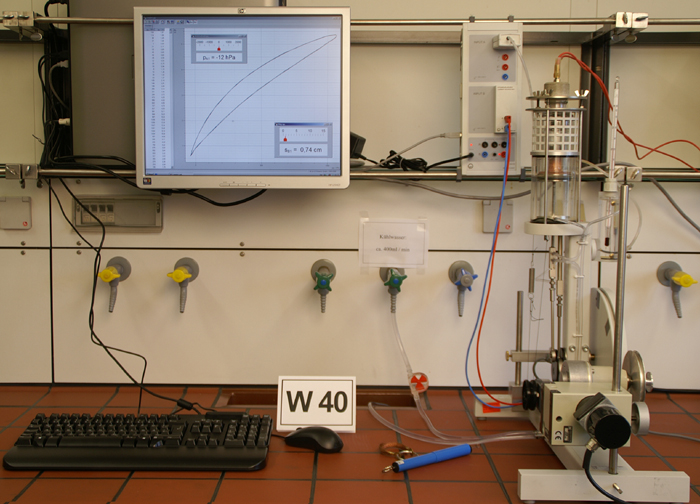
\includegraphics[width=0.75\textwidth]{Graphik/W40}
\caption{Versuchsskizze$^{\cite{A}}$}
\end{figure}

Für den Versuch werden folgende Geräte benötigt:
\begin{itemize}
\item Stirlingmotor
\item Reagenzglas mit Wasser (1 ml) 
\item Elektromotor
\item Drehzahlmesser
\item Glühwendel
\item Computer mit CassyLab
\item Regeltransformator für den Elektromotor und die Glühwendel
\end{itemize}
\newpage
Im ersten Versuchsteil wird das Reagenzglas auf den Stirlingmotor festgeschraubt und eine Messfühler für die Temperatur mittig ins Reagenzglas eingeführt. Dann wird das Schwungrad mit Hilfe des E-Motors in Uhrzeigersinn gedreht. Im zweiten Teil wird das Schwungrad dann einfach gegen den Uhrzeigersinn gedreht. \par

Im letzten wird das Reagenzglas mit Wasser ausgebaut und durch eine Heizwendel ersetzt. Der Heizstrom wird nun langsam erhöht, sodass sich mit einem kleinen Schubser das Schwungrad von Hand im Uhrzeigersinn drehen lässt.  

\subsection{Versuchsdurchführung}

Im ersten Teil des Versuchs beschleunigt der E-Motor das Schwungrad des Stirlingmotors. Im selben Moment soll mit Hilfe von CassyLab der Temperaturverlauf über die Zeit ermittelt werden. Dieser Teil des Versuchs wird solange durchgeführt bis das Wasser gefriert auf -10$^{\circ}$C gebracht wurde. \par

Im zweiten Teil des Versuchs wird nun wieder der zeitliche Verlauf der Temperatur gemessen, wobei bis auf eine Temperatur von etwas mehr als 37$^{\circ}$C erwärmt wird.\par

Im letzten Teil des Versuchs soll nun der Stirlingmotor auf eine Drehzahl von etwa 280 Umdrehungen Pro Minute kommen. Es wird ein PV-Diagramm erstellt mit Hilfe von CassyLab. Dann wird der Stirlingmotor auf eine Drehzahl von etwa 190 Umdrehungen Pro Minute gebremst und es wird wieder ein PV-Diagramm gemacht. Dasselbe wird wieder für eine neue Drehzahl wiederholt.
\noindent
\newpage


\section{Formeln}

\subsection{Schmelzwärme}
Für den Versuch ist die Berechnung der Schmelzwärme wichtig, dafür wird folgenden Formel verwendet:
\begin{equation}
Q_{\text{s}} = c_{\text{Stoff}}\cdot \frac{\Delta T}{\Delta t} \cdot t
\end{equation}
Wobei hier $c_{\text{Stoff}}$ die spezifische Wärmekapazität ist, welche im ersten Teil des Versuchs für Wasser genommen werden soll, im zweiten Teil für Eis. 
\subsection{Wirkungsgrade}
\begin{itemize}
\item Idealer Wirkungsgrade $\eta_{\text{ideal}}= \frac{T_1 -T_3}{T_1}$
\item effektiver Wirkungsgrad $\eta_{\text{eff}}= \frac{P_B}{P_e}$
\item Innerer Wirkungsgrad $\eta_{\text{i}}=\frac{P_{\text{ind}}}{P_e}$
\item mechanischer Wirkungsgrad $\eta_{\text{m}} = \frac{P_B}{P_{\text{ind}}}$
\end{itemize}
Hierbei sind 
\begin{align*}
P_{\text{ind}}& = \frac{A}{T_{\text{U}}} \\
P_B &= 2\pi \cdot  r \cdot F \cdot f
\end{align*}
hierbei ist $T_{\text{U}}$ die Umlaufdauer des Schwungrades, A die Fläche, welche in CassyLab gemessen wurde. $F$ ist die Bremskraft, $r=12\,\text{mm}$ der Radius des kleinen Kolbens und $f$ die Drehfrequenz.
\newpage
\section{ Messwerte}
\begin{figure}[H]
\centering
\caption{Messwerte }
\begin{tabular}{|c|c|c|} \hline
Umdrehung unbelastet [1/min] & Fläche A [hPacm$^3$] & Leistung P$_e$ [W] \\ \hline
283 & 22430 & 212 \\ \hline
246 & 19810 & 175  \\ \hline
\end{tabular}				 
\end{figure}
\begin{figure}[H]
\centering
\caption{Messwerte }
\begin{tabular}{|c|c|c|c|c|} \hline
Umdrehung belastet [1/min] & Fläche A [hPacm$^3$] & Motorkraft F$_K$ [N]  & Reibkraft F$_R$ [N]\\ \hline
190 & 25230 & 15,70 & 5,89 \\ \hline
155 &22870 & 15,5 &2,5 \\ \hline
\end{tabular}				 
\end{figure}


\section{ Auswertung}

Für das Temperatur-Zeit-Diagramm ergab sich folgendes:
\begin{figure}[H]
\centering
\includegraphics[width=0.75\textwidth]{Graphik/bla}
\caption{Temperatur-Zeit-Diagramm}
\end{figure}

\subsection{Schmelzwärme}

Im ersten Teil des Versuchs werden zuerst die Jeweiligen Steigungen der Geraden ermittelt, um $\frac{\Delta T}{\Delta t}$ zu ermitteln. In der nachfolgenden Tabelle werden alle wichtigen Werte für das errechnen von $\frac{\Delta T}{\Delta t}$ aufgelistet.
\begin{figure}[H]
\centering
\caption{Auswertung $\frac{\Delta T}{\Delta t}$}
\begin{tabular}{|c|c|c|c|c|} \hline
Anfangszeit	[s] & Anfangstemp. [$^{\circ}$C] & Endzeit [s] & Endtemp.  [$^{\circ}$C] & Steigung $\frac{\Delta T}{\Delta t}$ [$\frac{K}{s}$]  \\ \hline
11,12 & 23,43 & 210,67 & -6,37 & -0,15  \\ \hline
813,56 & -10,59 & 841,01 & 0,98 & 0,35\\ \hline
\end{tabular}				 
\end{figure}

Daraus ergeben sich folgende Schmelzwärmen:
\begin{align*}
Q_{\text{s}} &= c_{Wasser}\cdot \frac{\Delta T}{\Delta t} \cdot t = 4, 182\,\frac{\text{J}}{\text{g K}} \cdot \l(-0,15)\,\frac{\text{K}}{\text{s}}\r \cdot 240,67\,\text{s}\\
&= 132,153\,\frac{\text{J}}{\text{g}}= 132153\,\frac{\text{J}}{\text{kg}} 
\end{align*}
für $t=240,67\,\text{s}$ und $c_{Wasser}= 4, 182\,\frac{\text{J}}{\text{g K}}$ bei Wasser. $^{\cite{2}}$ Analog ergibt sich dann für Eis:
\begin{align*}
Q_{\text{s}} &= c_{Eis}\cdot \frac{\Delta T}{\Delta t} \cdot t = 2,220\,\frac{\text{J}}{\text{g K}} \cdot \l(0,35)\,\frac{\text{K}}{\text{s}}\r \cdot 841,01\,\text{s}\\
&= 653,464\,\frac{\text{J}}{\text{g}}= 653464\,\frac{\text{J}}{\text{kg}} 
\end{align*}
für $t=8410,1\,\text{s}$ und $c_{Eis}= 2,220\,\frac{\text{J}}{\text{g K}}$ bei Eis.  $^{\cite{2}}$
\newpage
\subsection{Bremsleistung und induzierte Leistung}

Aus dem Abschnitt Formeln wissen wir, dass für die Bremsleistung folgendes gilt:
\begin{align*}
P_{B_1} &= 2\pi \cdot  r \cdot F \cdot f = 2\pi \cdot 0,012\text{m} \cdot (15,70-5,86)\,\text{N} \cdot 190\,\frac{1}{60\text{s}} = 2,35\,\text{W}\\
P_{B_2} &=  2\pi \cdot  r \cdot F \cdot f = 2\pi \cdot 0,012\text{m} \cdot (14,50-2,50)\,\text{N} \cdot 155\,\frac{1}{60\text{s}} = 2,34\,\text{W}
\end{align*}
Für die induzierte Leistung ergibt sich:
\begin{align*}
P_{\text{ind}_1}& = \frac{A}{T_{\text{U}}} =\frac{2,523\,\text{J} \cdot 190 \,\text{s}}{60} = 7,99\,\text{W} \\
P_{\text{ind}_2}& = \frac{A}{T_{\text{U}}} =\frac{2,2870\,\text{J} \cdot 155 \,\text{s}}{60} =5,91\,\text{W} \\
\end{align*}

\subsection{Wirkungsgrade}

Zuguterletzt werden noch die Wirkungsgrade ausgerechnet für den Versuch, angefangen mit dem Idealen Wirkungsgrad:
\begin{align*}
\eta_{\text{ideal}}= \frac{T_1 -T_3}{T_1} = \frac{(830 -293)\,\text{K}}{830\,\text{K}} = 0,65
\end{align*}
wobei laut T(P$_e$)-Diagramm im Versuchsraum sich für 175 Watt eine Temperatur von $T_1$ = 830 Kelvin ergibt. Für das Kühlwasser wird eine Temperatur von  $T_2$ =293 Kelvin angenommen. Für ersten Versuch kann nichts ausgerechnet werden, da das T(P$_e$)-Diagramm nicht über 200 Watt geht. \par

Für den effektiven Wirkungsgrad gilt:
\begin{align*}
 \eta_{\text{eff}_1}&= \frac{P_{B_1}}{P_{e_1}} = \frac{2,35\,\text{W}}{212\,\text{W}} = 0,011 \\
  \eta_{\text{eff}_2}&= \frac{P_{B_2}}{P_{e_2}} = \frac{2,34\,\text{W}}{175\,\text{W}} = 0,013
\end{align*}
Hier lässt sich $ P_{e}$ aus den Messwerten ablesen und $P_B$ wurde vorhin ausgerechnet. \par

Nun geht es um den inneren Wirkungsgrad:
\begin{align*}
 \eta_{\text{i}_1}&=\frac{P_{\text{ind}_1}}{P_{e_1}} = \frac{7,99\,\text{W}}{212\,\text{W}}= 0,04 \\
  \eta_{\text{i}_2}&=\frac{P_{\text{ind}_2}}{P_{e_2}} = \frac{5,91\,\text{W}}{175\,\text{W}}= 0,03
\end{align*}

Zuletzt geht es noch um den mechanischen Wirkungsgrad:
\begin{align*}
\eta_{\text{m}_1} &= \frac{P_{B_1}}{P_{\text{ind}_1}}= \frac{2,35\,\text{W}}{7,99\,\text{W}} = 0,29 \\
  \eta_{\text{m}_2}&= \frac{P_{B_2}}{P_{\text{ind}_2}} = \frac{2,34\,\text{W}}{5,91\,\text{W}} = 0,395
\end{align*}
Hier lässt sich nun eine Probe machen, denn:
\begin{align*}
\eta_{\text{m}}=\frac{ \eta_{\text{eff}}}{ \eta_{\text{i}_1}}
\end{align*}
Draus ergibt sich hier:
\begin{align*}
\eta_{\text{m}_1}&=\frac{ \eta_{\text{eff}_1}}{ \eta_{\text{i}_1}} = \frac{0,011}{0,04}= 0,275\\
\eta_{\text{m}_2}&=\frac{ \eta_{\text{eff}_2}}{ \eta_{\text{i}_2}} = \frac{0,013}{0,03}= 0,433
\end{align*}
Dadurch sieht man, dass der Versuch ungenau ist, worauf in der Fehlerdiskussion eingegangen wird.
\newpage
\subsection{P-V-Diagramme}

\begin{figure}[H]
\centering
\includegraphics[width=0.75\textwidth]{Graphik/bla1}
\caption{P-V-Diagramm}
\end{figure}
\begin{figure}[H]
\centering
\includegraphics[width=0.75\textwidth]{Graphik/bla2}
\caption{P-V-Diagramm}
\end{figure}
Laut Auswertung von CassyLab, geschieht die belasteten Fälle mehr Leistung. Das sieht man vorallem in Abbildung 7 durch die größere eingeschlossene Fläche ersichtlich. Ebenfalls in Abbildung 7 sieht man, dass die Peakpunkte relativ nah aneinander sind. In Abbildung 6 verschiebt sich der belastete Fall um 10\,hPa, was ich mir aber nicht erklären kann. 

\section{Fehlerdiskussion}

In diesem Versuch hat viele Fehlerquellen. Zum einen sind alle Messgeräte mit Messtoleranzen verbunden. Des weiteren wird bei diesem Versuch angenommen, dass die abgeführte Wärmemenge pro Zeit konstant sei. Zwischen ersten und zweiten Teil des Versuchs wird die Laufrichtung geändert. Dazu wird kurz die Drehzahl runtergedreht und wieder rauf. Dies wird allerdings in diesem Versuch vernachlässigt.  Bei der Bestimmung der Bremskraft ist es zudem nicht einfach, konstant auf eine Drehzahl herunterzubringen, das führt vor allem bei der Bremsleistung zu relativ großen Fehlern. Ein letzte Fehler ist, dass beim erwärmen des Wasser Eisstücke dann im Wasser rumschwimmen können. Diese Berühren dann den Fühler und ergeben Fehler in dem Temperatur Zeit Diagramm, wie zwischen 900 und 100 Sekunden zu sehen ist.


\section{Zusammenfassung}

Im Grunde hatte der Versuch zwei Ziele. Zum einen die Berechnung der Schmelzwärme und zum einen die Wirkungsgrade.
Für die Schelzwärme ergibt sich folgendes:
\begin{itemize}
\item  Für den Vorgang Wasser zu Eis erhält man eine Schmelzwärme von $Q_{\text{s}} = 132153\,\frac{\text{J}}{\text{kg}} $ 
\item Für den Vorgang Eis zu Wasser erhält man eine Schmelzwärme von  $Q_{\text{s}} = 653464\,\frac{\text{J}}{\text{kg}} $
\end{itemize}
Die verschiedenen Wirkungsgrade sind in diesem Versuch: 

\begin{figure}[H]
\centering
\caption{Wirkungsgrade}
\begin{tabular}{|l|c|c|c|c|} \hline
Wirkungsgrad & erste Messung & zweite Messung\\\hline
effektiven Wirkungsgrad & 0,011 &  0,013 \\\hline
inneren Wirkungsgrad & 0,04 & 0,03\\\hline
mechanischen Wirkungsgrad& 0,29 & 0,395\\\hline
\end{tabular}				 
\end{figure}
Für den zweiten Versuch erhält man zudem noch $\eta_{\text{ideal}} = 0,65$
\newpage
\section{Literaturverzeichnis}

\renewcommand{\refname}{~}
\vspace{-30pt}
\begin{thebibliography}{xx}

   \bibitem[1]{1}  	\textit{\glqq  W40 Heißluftmotor\grqq , in 	\\
   					http://www3.physik.uni-stuttgart.de/studium/praktika/ap/}, \\
   					unter \textit{http://www3.physik.uni-stuttgart.de/studium/praktika/ap/pdf\_dateien/W40.pdf}; \\
   								abgerufen am 07.10.2015
   	 \bibitem[2]{2}  	\textit{\glqq Literaturwert spezifische Wärmekapazität\grqq } unter 	
   					\textit{https://elearning.physik.\\uni-frankfurt.de/data/FB13-PhysikOnline/lm\_data/lm\_282/auto/anhang1/cd425.htm}; \\
   								abgerufen am 07.10.2015							
   \bibitem[A]{A}  	Graphik aus \textit{\glqq  W40 Heißluftmotor\grqq , in 	\\
   					http://www3.physik.uni-stuttgart.de/studium/praktika/ap/}, \\
   					unter \textit{http://www3.physik.uni-stuttgart.de/studium/praktika/ap/pdf\_dateien/W40.pdf}; \\
   								abgerufen am 06.10.2015
\end{thebibliography}

\section{Anhang}

\end{document}